\documentclass[10pt,letterpaper]{article}
\usepackage[utf8]{inputenc}
\usepackage[spanish,es-tabla]{babel}
\spanishdecimal{.}
\usepackage{amsmath}
\usepackage{amsfonts}
\usepackage{amssymb}
\usepackage{makeidx}
\usepackage{graphicx}
\usepackage{kpfonts}
\usepackage{listings}
%\usepackage{fontspec}
\usepackage{float}
\usepackage{siunitx} %Para el simbolo de ohm
\usepackage{enumerate}
\usepackage{array}
\usepackage{multicol}
\usepackage{multirow}
\usepackage{colortbl}
\usepackage{pdfpages}
\usepackage{subfigure}
\begin{document}
    \begin{titlepage}
     \centering
	   \begin{figure}
            \begin{minipage}{1\linewidth}
            \centering\centering%\rule{2cm}{2cm}
%              \caption{Primera figura}
            \includegraphics[width=0.3\textwidth]{C:/Users/anton/Documents/MCIA/UAQ _MCIA/Sem2_Computo_Evolutivo/Pictures/logos_fi_uaq.png}
            \end{minipage}
        \end{figure}
        
        {\scshape\LARGE Universidad Autónoma de Querétaro \par}
	        \vspace{1cm}
	        
	    {\scshape\Large División de Investigación y Posgrado \par}
	        \vspace{1cm}
	        
		{\huge\bfseries Computo Evolutivo\par}
		    \vspace{1cm}
		    
		{\huge\bfseries Practica 4 \par}	
		    \vspace{1cm}
		    
		{\Large\itshape Problema TSP Restrictivo\par}
		    \vspace{1cm}
		    
		Profesor: Dr. Marco Antonio Aceves Fernández \par
		\vspace{1.2cm}
		
		Presenta:\par  \vspace{0.15cm}
		
        Ing. Osmar Antonio Espinosa Bernal
        
		\vfill
		% Bottom of the page
		{\large  06 de octubre de 2021\par}
		%{\large 10 de Octubre del 2019\par}
    \end{titlepage}
    	%\tableofcontents
		%\listoffigures
		%\listoftables
		\printindex
		
\section{Objetivo}
Desarrollar algoritmo que permita encontrar la ruta mas corta que recorra
todas y cada una de las diferentes ciudades mostradas en la tabla 1.

\begin{table}[H]
	\begin{center}
		\begin{tabular}{|c | l |}
			\hline
			City No. & City Name \\
\hline
\hline
1 & Berlin \\
\hline
2 & Hamburg \\
\hline
3 & Stuttgart \\
\hline
4 & Munich \\
\hline
5 & Paris \\
\hline
6 & Lyon \\
\hline
7 & Bordeaux \\
\hline
8 & Toulouse \\
\hline
9 & Amsterdam \\
\hline
10 & Brussels \\
\hline
11 & Luxemburg \\
\hline
12 & Zurich \\
\hline
13 & Geneva \\
\hline
14 & Vienna \\
\hline
15 & Linz \\
\hline
16 & Rome \\
\hline
17 & Florencia \\
\hline
18 & Naples \\
\hline
		\end{tabular}
		\caption{Listas de ciudades para TSP Restringido}
	\end{center}
\end{table}

\section{Marco Teórico}
El problema del agente viajero o TSP es un problema que pertenece a la clase de problemas NP-Duros debido a que no existe un algoritmo exacto que lo resuelva en tiempo polinomial. La importancia del TSP se estriba en que varios problemas de optimización combinatoria se pueden modelar con base en él, como la planeación de rutas de transporte, el taladrado en placas de circuitos, la planeación de tiempos de vuelos y la asignación de tareas, así como otros que pueden ser consultados. Existen métodos conocidos como Metaheurísticas los cuales son algoritmos aproximados que se pueden adaptar a varios problemas de optimización.
\\\\
El problema fue formulado por primera vez en 1930 y es uno de los problemas de optimización más estudiados. Es usado como prueba para muchos métodos de optimización. Aunque el problema es computacionalmente complejo, se conoce gran cantidad de heurísticas y métodos exactos, así que es posible resolver planteamientos concretos del problema desde cien hasta miles de ciudades.
\\\\
\textbf{\large Algoritmos genéticos} 
\\\\
Los algoritmos genéticos parten de la premisa de emplear la evolución natural
como un procedimiento de optimización que se caracteriza por tener operaciones básicas que son:

\begin{itemize}
\item Selección de cromosomas
\item Cruzamiento de cromosomas
\item Mutación de cromosomas
\end{itemize}

Por lo tanto, el algoritmo es una búsqueda empleando dichas operaciones; por ejemplo, se puede plantear una familia de individuos los cuales se seleccionan y después se considera a los mas óptimos para realizar un cruzamiento entre ellos, y la forma de evitar caer en mínimos locales es el empleo de la mutación. Por ello la mutación puede considerarse una operación de fuga de mínimos locales. Esta búsqueda se define como una búsqueda de un espectro amplio.
\\\\
\textbf{\large Métodos de Selección de cromosomas}
\\\\
\begin{itemize}
\item \textbf{Selección por torneo:} se eligen subgrupos de individuos de la población, y los miembros de cada subgrupo compiten entre ellos. Sólo se elige a un individuo de cada subgrupo para la reproducción.

\item \textbf{Selección Rank:} a cada individuo de la población se le asigna un rango numérico basado en su aptitud, y la selección se basa en este ranking, en lugar de las diferencias absolutas en aptitud. 

\end{itemize}

Estos son los tipos de seleccion de cromosomas que se eligen para la presente practica.
\\\\
\hrulefill \textbf{\large Cruzamiento de cromosomas}
\\\\
El cruce parcialmente mapeado (PMX) fue propuesto por Goldberg y Lingle[1]. Seleccionados 2 cromosomas, este cruce realiza 2 cortes en el cromosoma 1 aleatoriamente y lo coloca en el descendiente 2 en la posición elegida para corte. Lo mismo sucede con el cromosoma 2 y lo asigna al descendiente 1. Como se observa a continuación:

\[C_1 = ( 3 4 8 | 2 7 1 | 6 5 )\]
\[C_2 = ( 4 2 5 | 1 6 8 | 3 7 )\]\\
\[D_1 = ( x x x | 1 6 8 | x x )\]
\[D_2 = ( x x x | 2 7 1 | x x )\]

Después se buscan los genes faltantes buscando en la matriz de correspondencia del descendiente 1 para el descendiente 2 y viceversa. También se comprueba que el gen a intercambiar no se encuentra ya en el nuevo descendiente, se procede a su llenado como sigue:

\[D_1 = ( 3 4 x | 1 6 8 | x 5 )\]
\[D_2 = ( 4 x 5 | 2 7 1 | 8 x )\]

Finalmente se mapean los genes que ya tienen un gen igual y lo intercambian por su correspondiente en la matriz de correspondencia, quedando los descendientes como sigue:

\[D_1 = ( 342 | 1 6 8 | 75 )\]
\[D_2 = ( 485 | 2 7 1 | 36 )\]

El operador de cruce de órdenes (OX) fue propuesto por Davis[2]. Este cruce hace 2 cortes definidos de forma aleatoria a los 2 cromosomas que se desean cruzar y se pasan al los descendientes manteniendo sus posiciones o eligiendo uno aleatorio. Después se mantiene el orden de los cromosomas donde finalizo el corte se procede a inserta siguiendo ese mismo orden evitando insertar los genes ya presentes en el descendiente. De esta manera se evitan duplicados, como se muestra a continuación. 

\[C_1 = ( 3 4 8 | 2 7 1 | 6 5 )\]
\[C_2 = ( 4 2 5 | 1 6 8 | 3 7 )\]\\
\[D_1 = ( x x x | 2 7 1 | x x )\]
\[D_2 = ( x x x | 1 6 8 | x x )\]

Ahora, la secuencia a partir del segundo corte del cromosoma 2 es: 3, 7, 4, 2, 5, 1, 6, 8. Eliminando los genes ya presentes en el descendiente 1, queda: 3, 4, 5, 6, 8. El descendiente 2 se construye análogamente, por lo tanto los descendientes quedan de la siguiente manera:

\[D_1 = ( 568 | 271 | 34 )\]
\[D_2 = ( 427 | 168 | 53 )\]
\\\\
\hrulefill \textbf{\large Mutación}
\\\\
La mutación en los algoritmos se utiliza para evitar que los algoritmos genético caigan en mínimos locales, esto al realizar cambios a cromosomas seleccionados que dan la oportunidad de hacer nuevas búsquedas para mejorar o cambiar la descendencia. Generalmente se le aplica a los individuos de una población procurando que no exceda el 10\% de la población total.
\\\\
\textbf{\large Mutación Scramble 2}
\\\\
Esta mutación se realiza haciendo un corte en 2 puntos en un  cromosoma elegido aleatoriamente, después los genes restante en el cromosoma se juntan, formando un subcromosoma, finalmente la sección cortada se realiza un cambio de posición de sus genes evitando que queden en su ubicación original. Para terminar de completar la mutación, se re-inserta la sección mutada de nuevo a la sección donde se juntaron los genes originales de forma aleatoria, como se muestra a continuación:

\[D_1 = ( \;5\;6\;8\; |\; 2\;7\;1\; | \;3\;4\; )\]
\[D_2 = ( \;4\;2\;7 \;|\; \;1\;6\;8\; |\; 5\;3\; )\]

\[D_1 = ( \;5\;6\;8\;3\;4\; )\]
\[D_2 = ( \;4\;2\;7\;5\;3\; )\]

\[D_1 = (\;2\;7\;1\;)\]
\[D_2 = (\;1\;6\;8\;)\]

\[D_1 = (\;1\;2\;7\;)\]
\[D_2 = (\;8\;1\;6\;)\]

\[D_1 = ( \;5\;|\;1\;2\;7\;|\;6\;8\;3\;4\; )\]
\[D_2 = ( \;4\;|\;8\;1\;6\;|\;2\;7\;5\;3\; )\]

\section{Materiales}
Computadora personal portátil MSI, procesador Intel(R)Core(TM) i7-750H CPU @ 2.60GHz, 16GB de memoria RAM, Sistema operativo Windows 10 de 64 bits, Software: Jupyter Notebook y entorno Anaconda, lenguaje Python.

\section{Metodología}
El algoritmo desarrollado es como sigue:
\\\\
\hrulefill \textit{Creación de una población aleatoria de cromosomas} \\
\hspace*{1cm}\textit{Validación de cromosomas}\\
\textit{Evaluación cromosomas}\\
\textit{Ordenación por criterio elitista}\\
\textit{Selección tipo de selección}\\
\textit{Selección tipo de cruza}\\
\textit{Selección tipo de mutación}\\
\textit{for epsilon $<$90\% or iteración $>$ a Generaciones}\\
\hspace*{1cm}\textit{Llamada a cruza}	\\
\hspace*{2cm}\textit{Validación de cromosomas}\\
\hspace*{1cm}\textit{Llamada a mutación}	\\
\hspace*{2cm}\textit{Validación de cromosomas}\\
\hspace*{1cm}\textit{Evaluación}	\\
\hspace*{1cm}\textit{Recopilación de datos de interés}	\\
\hspace*{1cm}\textit{Iteración + 1}	\\
\textit{Graficación de resultados}\\
\textit{Fin}\\
\\\\
Dado que unas ciudades no pueden ser directamente visitadas por otras ciudades, entonces se hace una validación de cromosomas cada vez que hay una modificación. Estos se producen durante la creación, la cruza y la mutación de los cromosomas.
\\\\
Para realizar la validación, se verifica que la cadena no contenga 'ND' cuando se revisa su respectiva distancia de una ciudad a otra. Los cromosomas validos se muestran en la figura 1.

\begin{figure}[H]
	\centering
    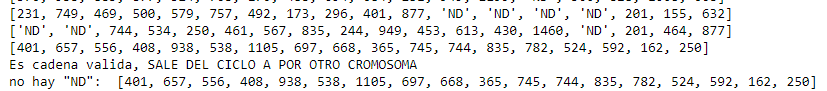
\includegraphics[width=1\textwidth]{C:/Users/anton/Documents/MCIA/UAQ _MCIA/Sem2_Computo_Evolutivo/Prac04TSPRestrictivo/pngs/CromValido.png}
    \caption{Cadena de genes validos.}
\end{figure}

Esta validación se realiza con el método \textit{if 'ND' not in cadena}  integrada en python.
\\\\
De igual manera, para asegurar la validez de un cromosoma se hace la mutación y cruza de manera aleatoria cada vez que busca un cromosoma, esto es, el tamaño de corte de genes y el indice de la sección donde cortara al cromosoma, en caso de no encontrar validos, vuelve a seleccionar valores aleatorios, la sección de código de la figura 2 muestra como determina de manera aleatoria los nuevos indices y sección de corte.

\begin{figure}[H]
	\centering
    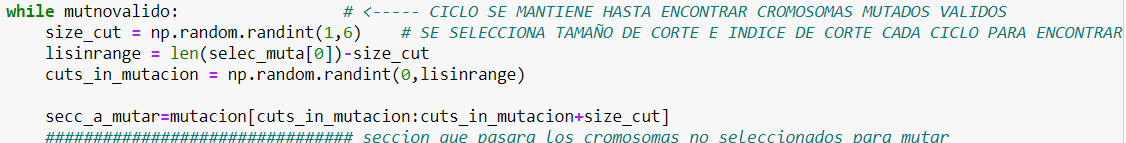
\includegraphics[width=1\textwidth]{C:/Users/anton/Documents/MCIA/UAQ _MCIA/Sem2_Computo_Evolutivo/Prac04TSPRestrictivo/pngs/aleatorios.png}
    \caption{Cadena de genes validos.}
\end{figure}

\section{Resultados y discusión}

\textbf{\large Prueba 1}
\\\\
Población inicial: 50 y 100 cromosomas\\
Selección Torneo y Selección Rank\\
Cruza PMX (Partially Mapped Crossover Operator)\\
Mutación Scramble\\
Generaciones: 150\\\\

En la gráfica de la figura 3 se observa la evolución de los cromosomas con una población inicial de 50 y 100 hasta encontrar una ruta que sea la mas corta posible y la media por generación.

\begin{figure}[H]
      \begin{center}
        \subfigure[Seleccion Torneo]{
            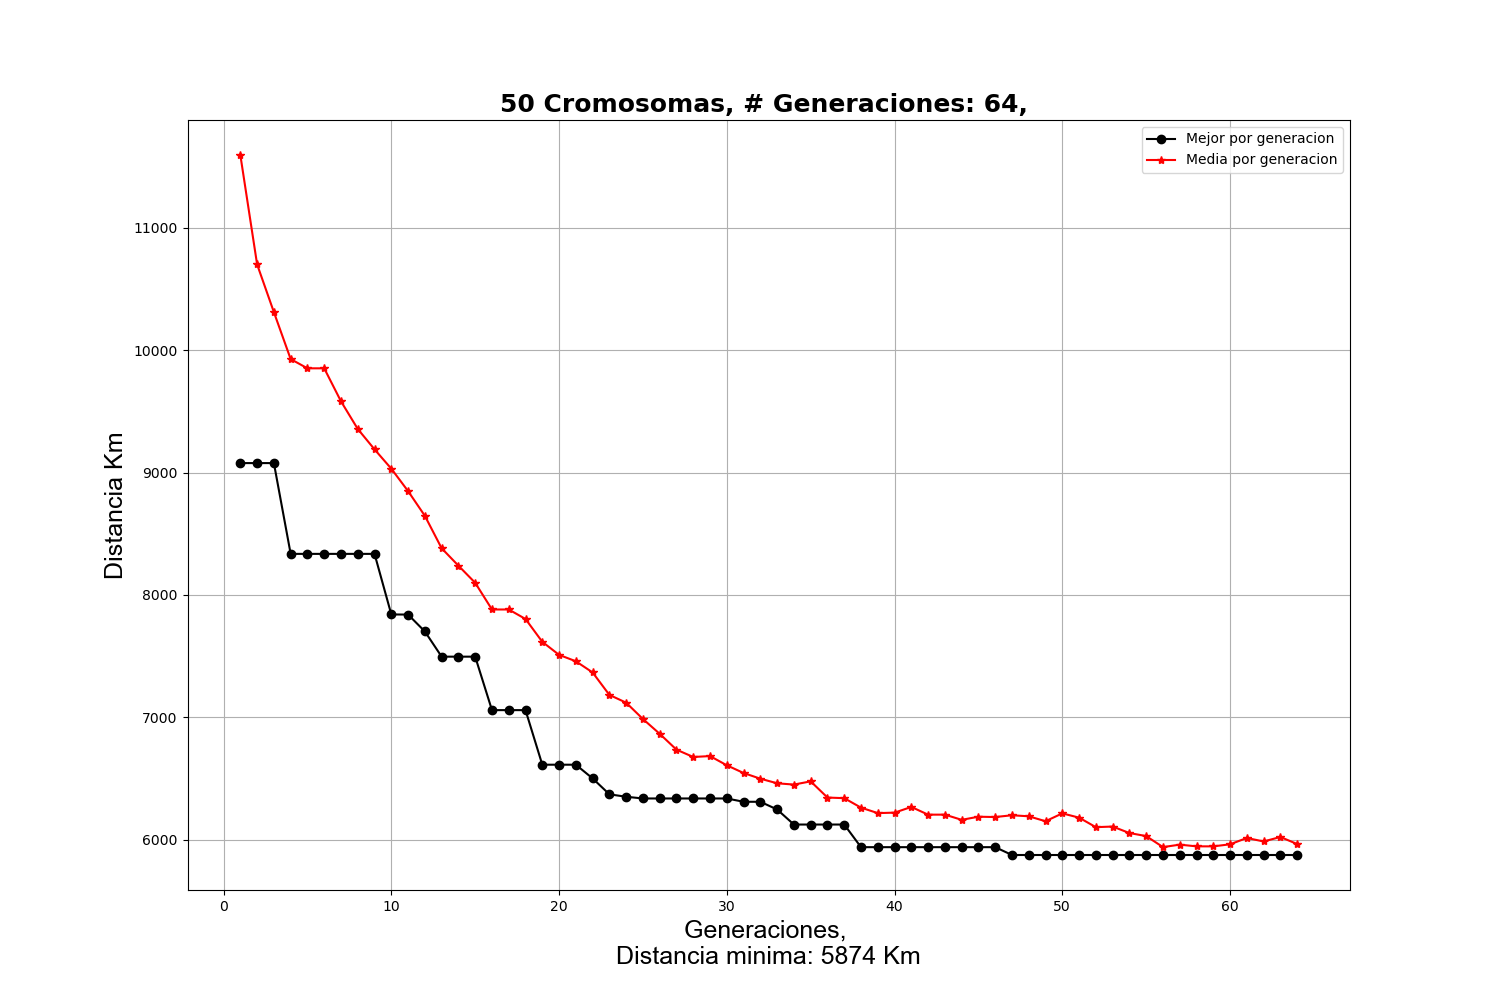
\includegraphics[width=0.47\textwidth]{C:/Users/anton/Documents/MCIA/UAQ _MCIA/Sem2_Computo_Evolutivo/Prac04TSPRestrictivo/pngs/Graf01.png}
            \label{Señal 1}}
        \subfigure[Seleccion Rank]{
            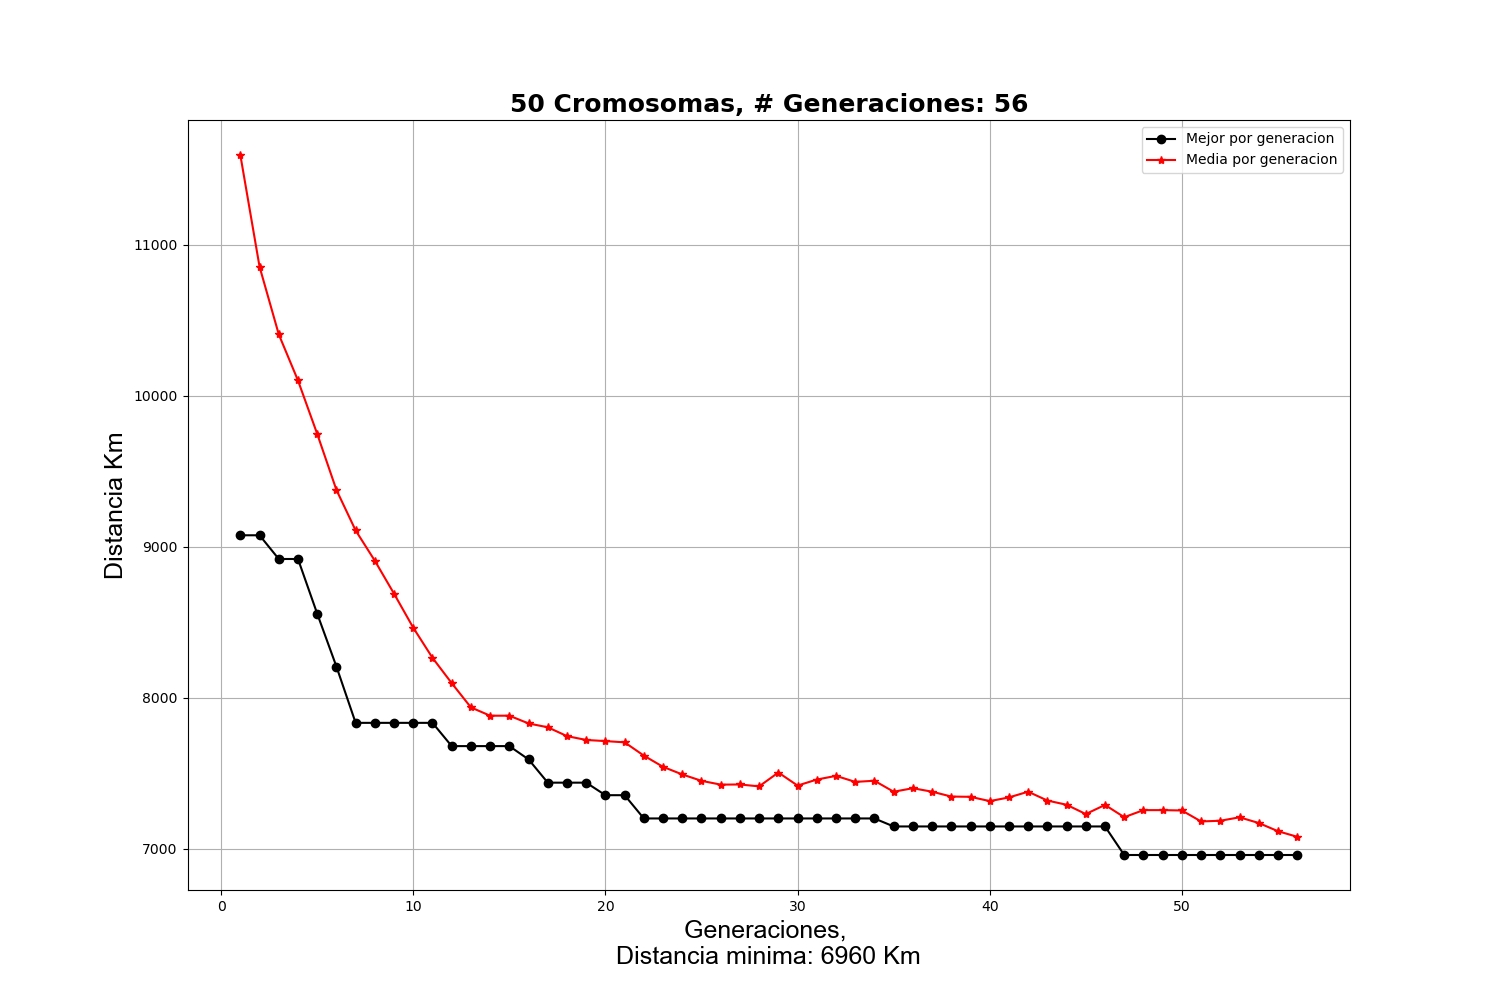
\includegraphics[width=0.47\textwidth]{C:/Users/anton/Documents/MCIA/UAQ _MCIA/Sem2_Computo_Evolutivo/Prac04TSPRestrictivo/pngs/Graf02.png}
            \label{Señal 2}}
        \subfigure[Seleccion Torneo]{
            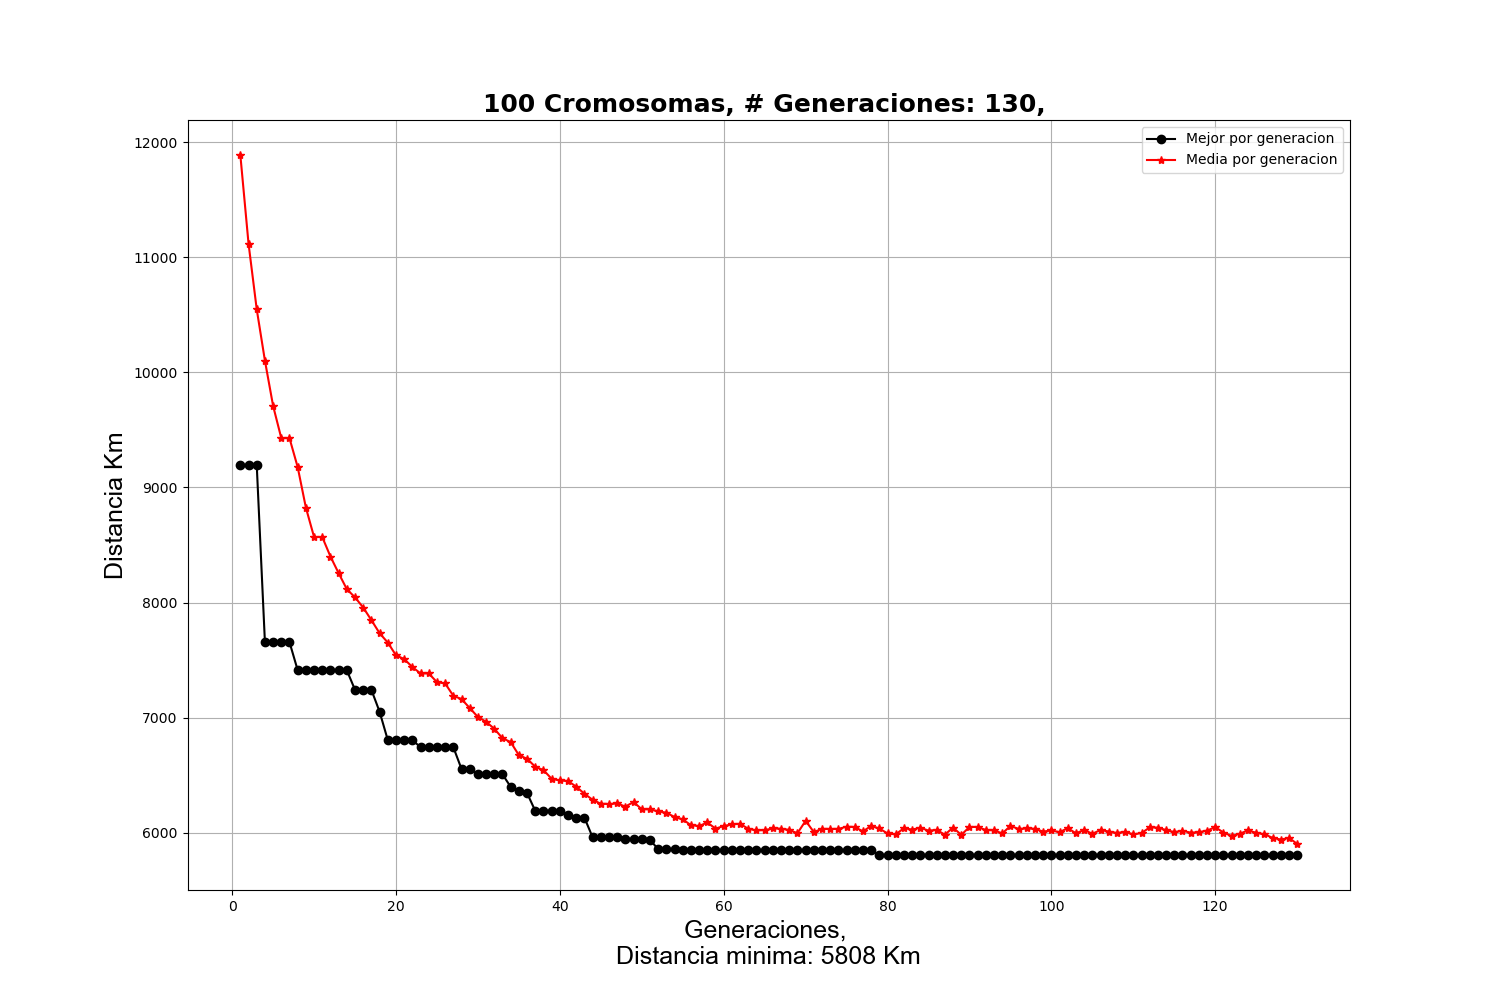
\includegraphics[width=0.47\textwidth]{C:/Users/anton/Documents/MCIA/UAQ _MCIA/Sem2_Computo_Evolutivo/Prac04TSPRestrictivo/pngs/Graf03.png}
            \label{Señal 2}}
        \subfigure[Seleccion Rank]{
            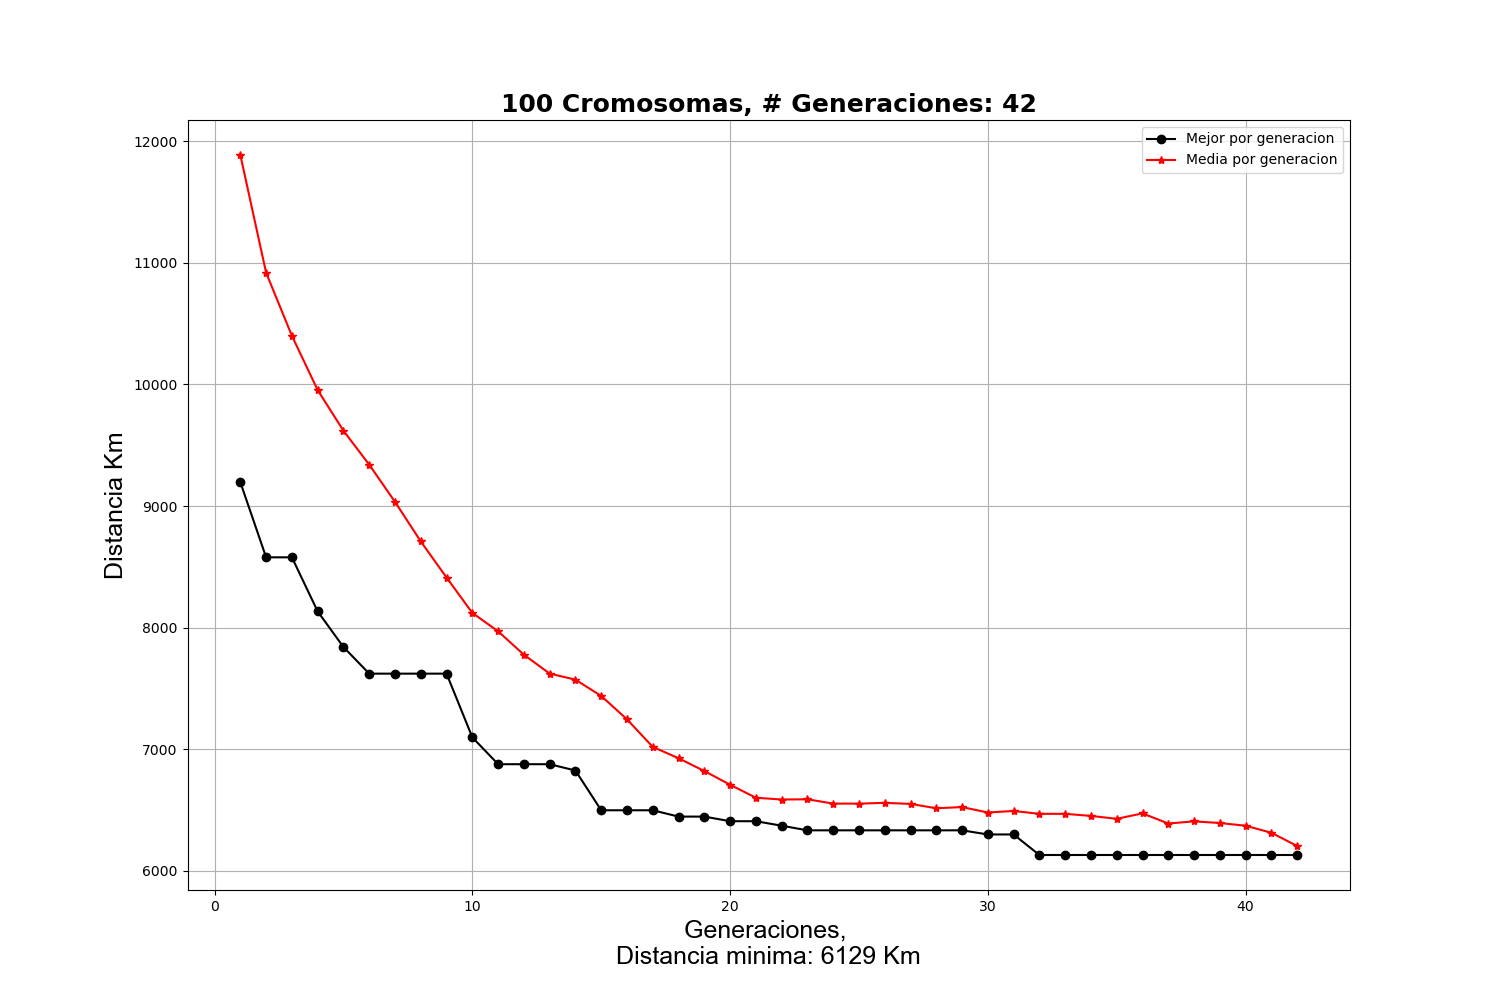
\includegraphics[width=0.47\textwidth]{C:/Users/anton/Documents/MCIA/UAQ _MCIA/Sem2_Computo_Evolutivo/Prac04TSPRestrictivo/pngs/Graf04.png}
            \label{Señal 2}}
        \caption{Comparación de Resultados con 50 y 100 cromosomas}
        \label{Patron de señales para reconocimiento de señal Gaussiana}
      \end{center}
    \end{figure}

Cuando se observan las gráficas se aprecia que la cantidad de cromosomas y el tipo de selección define la rapidez de encontrar tanto la distancia mas corta como el numero de iteraciones mas bajo para alcanzar dicha distancia corta. Sin embargo, no siempre se cumple ya que algunas veces, aunque alcanza el mínimo de distancia la mayoría de los cromosomas, la distancia es no es tan baja. Sin embargo el uso del selección PMX ofrece resultados mas bajos y en menos generaciones.

\textbf{\large Prueba 2}
\\\\
Población inicial: 50 y 100 cromosomas\\
Selección Torneo y Seleccion Rank\\
Cruza OX (Order Crossover Operator)\\
Mutación Scramble\\
Generaciones: 150\\\\

En la gráfica de la figura 4 se observa la evolución de los cromosomas con una población inicial de 50 y 100 hasta encontrar una ruta que sea la mas corta posible y la media por generación utilizando el método de selección OX (Order Crossover Operator).

\begin{figure}[H]
      \begin{center}
        \subfigure[Seleccion Torneo]{
            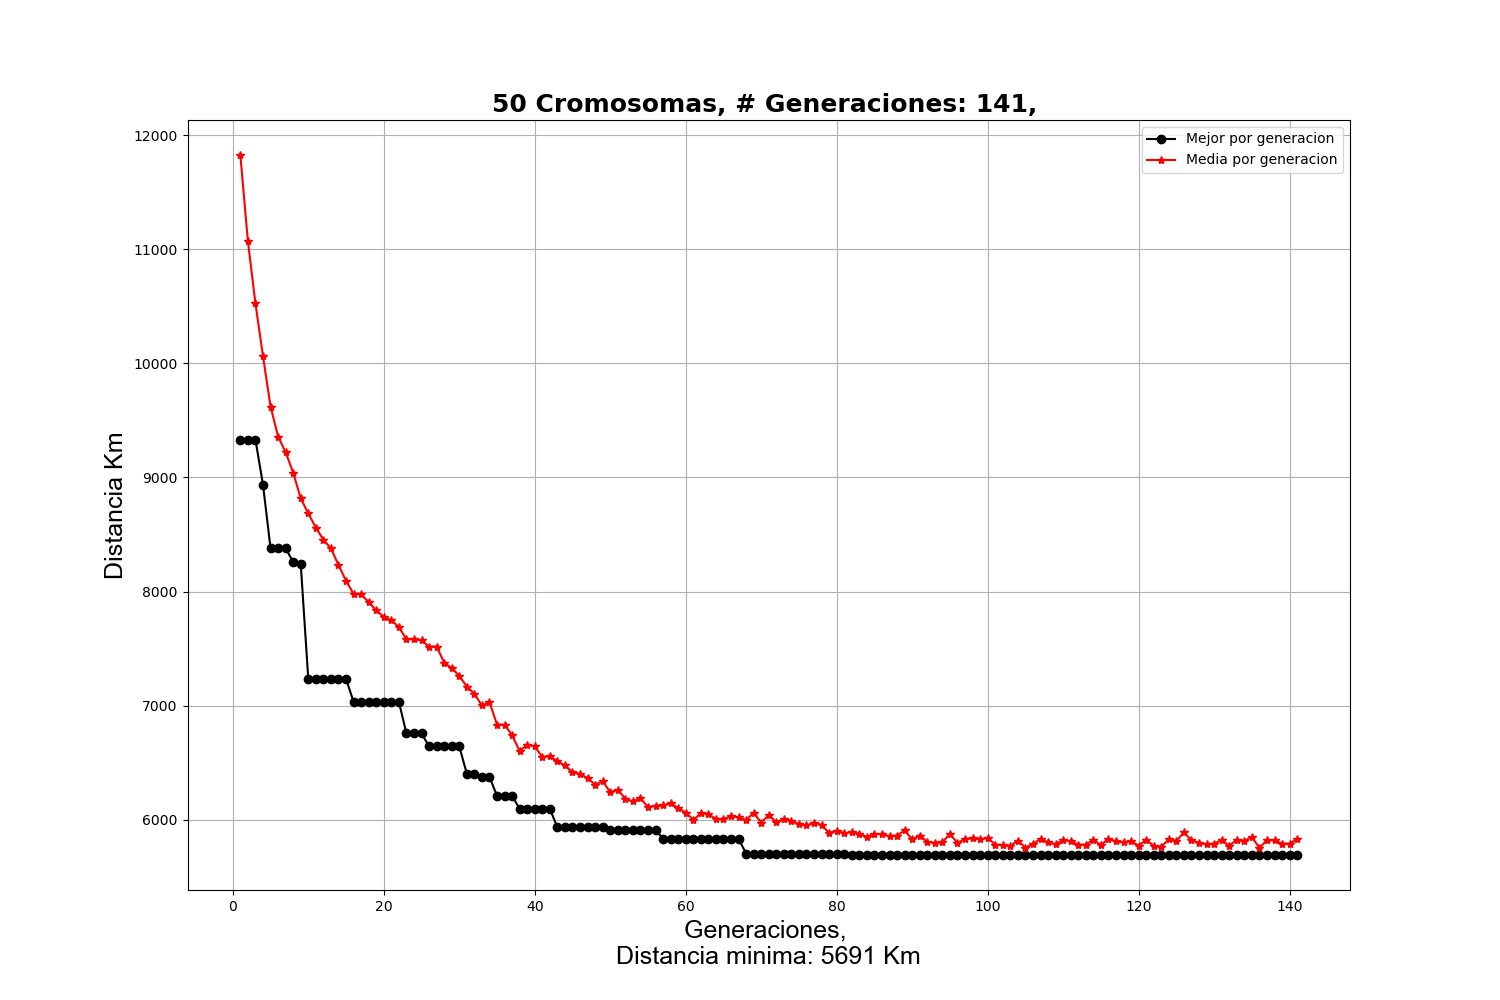
\includegraphics[width=0.47\textwidth]{C:/Users/anton/Documents/MCIA/UAQ _MCIA/Sem2_Computo_Evolutivo/Prac04TSPRestrictivo/pngs/Graf05.png}
            \label{Señal 1}}
        \subfigure[Seleccion Rank]{
            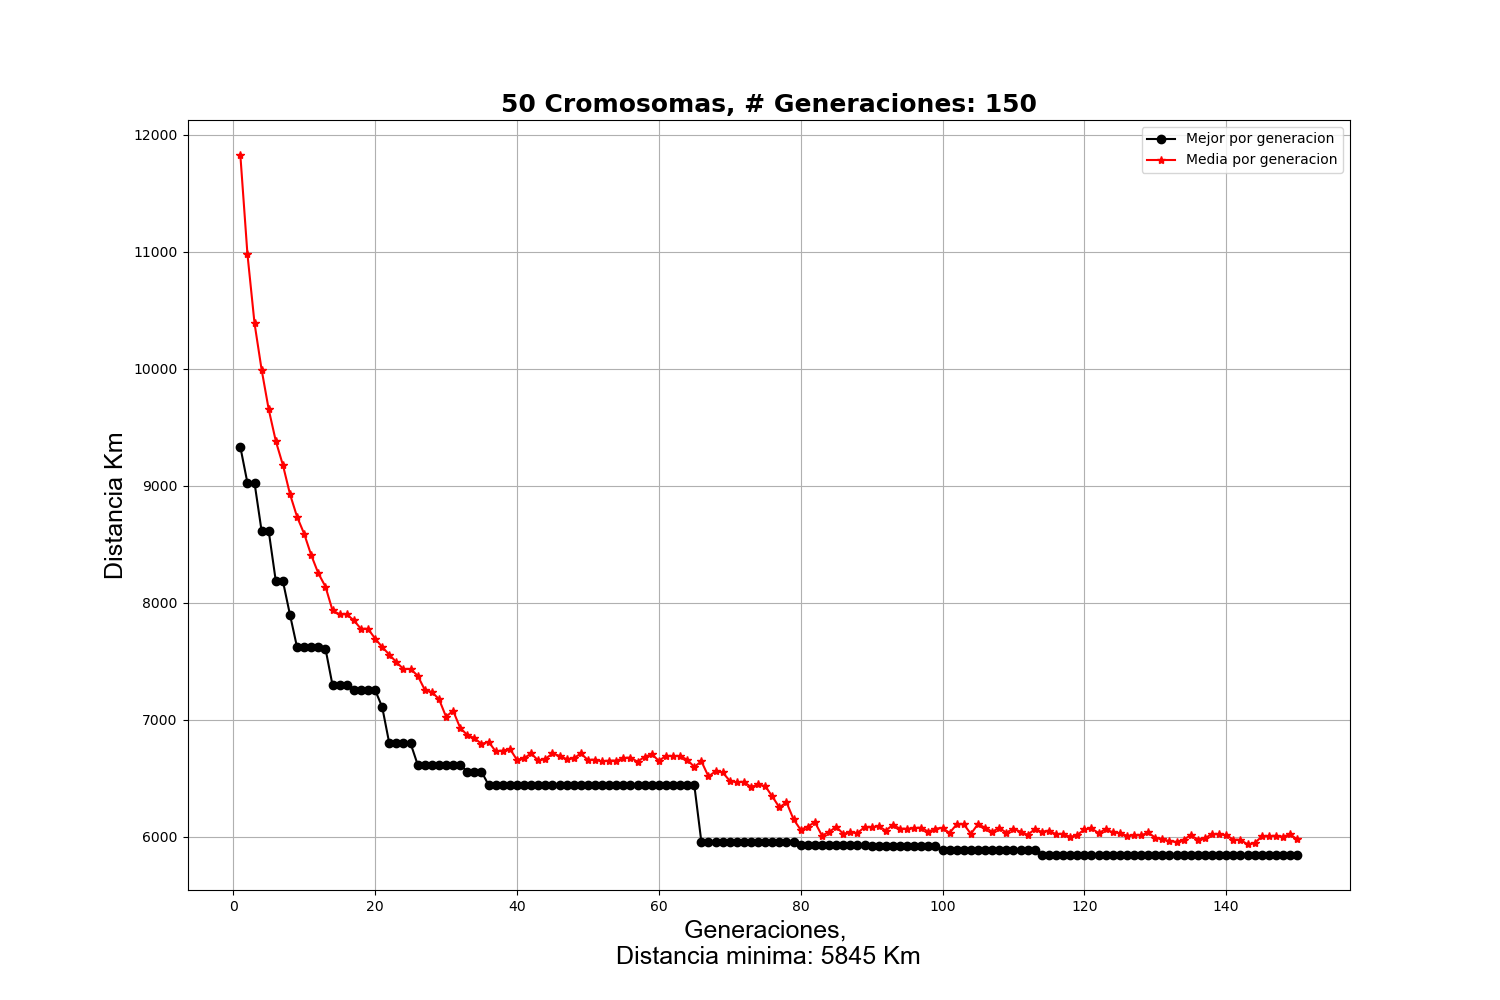
\includegraphics[width=0.47\textwidth]{C:/Users/anton/Documents/MCIA/UAQ _MCIA/Sem2_Computo_Evolutivo/Prac04TSPRestrictivo/pngs/Graf06.png}
            \label{Señal 2}}
        \subfigure[Seleccion Torneo]{
            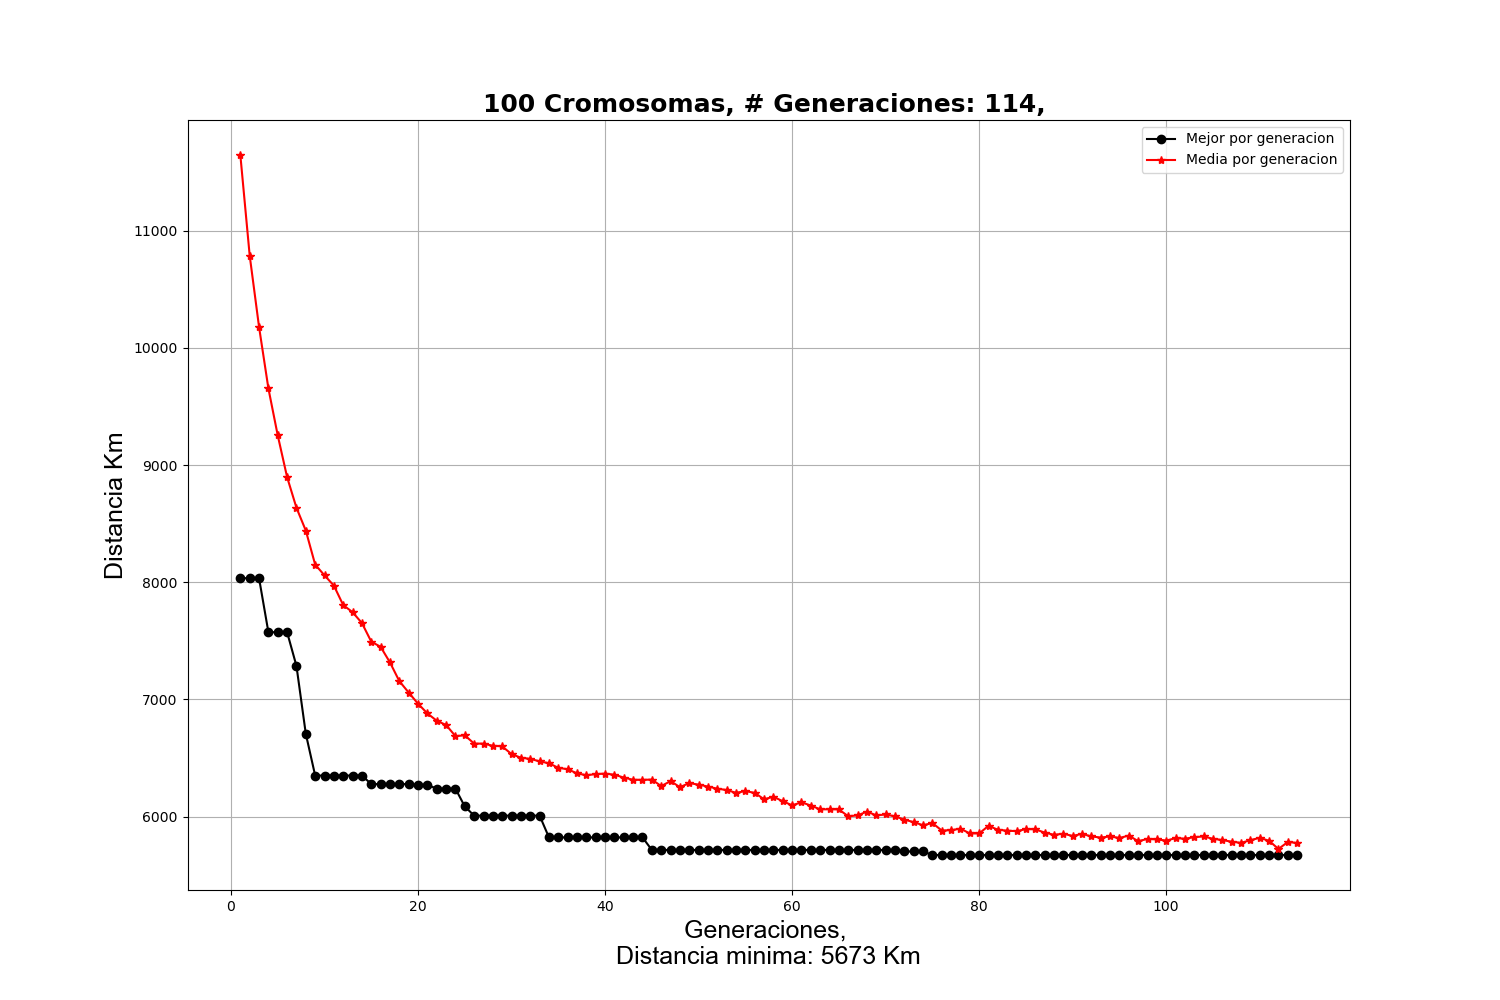
\includegraphics[width=0.47\textwidth]{C:/Users/anton/Documents/MCIA/UAQ _MCIA/Sem2_Computo_Evolutivo/Prac04TSPRestrictivo/pngs/Graf07.png}
            \label{Señal 2}}
        \subfigure[Seleccion Rank]{
            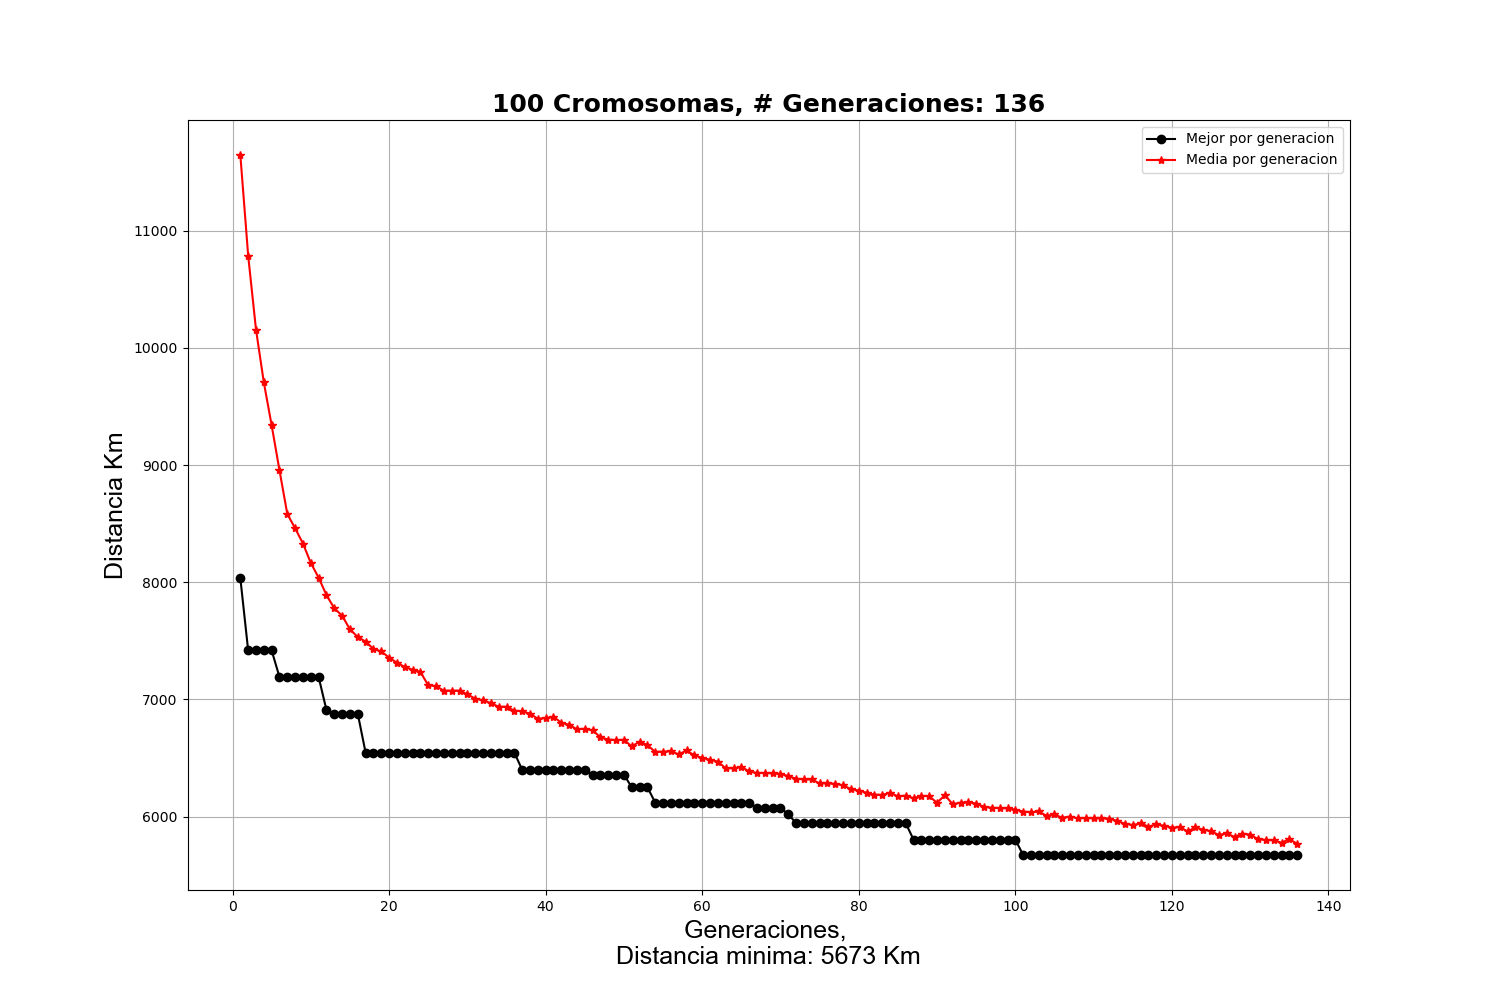
\includegraphics[width=0.47\textwidth]{C:/Users/anton/Documents/MCIA/UAQ _MCIA/Sem2_Computo_Evolutivo/Prac04TSPRestrictivo/pngs/Graf08.png}
            \label{Señal 2}}
        \caption{Comparación de Resultados con 50 y 100 cromosomas}
        \label{Patron de señales para reconocimiento de señal Gaussiana}
      \end{center}
    \end{figure}

Con selección OX se observa que le toma mas generaciones alcanzar una valor de distancia mínimo, ademas de que la media le cuesta mas conseguir un valor promedio estable, sin embargo un numero mayor de cromosomas le ayuda a disminuir las generaciones para encontrar un mínimo, aunque no lo suficiente.

\section{Conclusiones}
Cuando se trabaja con algoritmos de búsqueda de rutas con restricciones, los algoritmos de cruzamiento y mutación se enfrentan al desafió de encontrar combinaciones de cromosomas validos ademas de el tiempo necesario para encontrarlos, y que no contengan dichas restricciones, sin embargo una vez realizado no se observa diferencia alguna con la búsqueda tradicional, ya que cumple con el objetivo de encontrar la ruta mas corta posible. Sin embargo algunos algoritmos de cruza y mutación pueden tener problemas si no se desarrollan adecuadamente ya que pueden producir cromosomas no validos.
\\\\
En las figuras 5 y  6 se muestran los recorridos para la selección Torneo y Rank mas corto obtenido, el punto rojo indica el inicio del camino y el punto negro, la ciudad antes de volver al inicio de la ruta.

\begin{figure}[H]
	\centering
    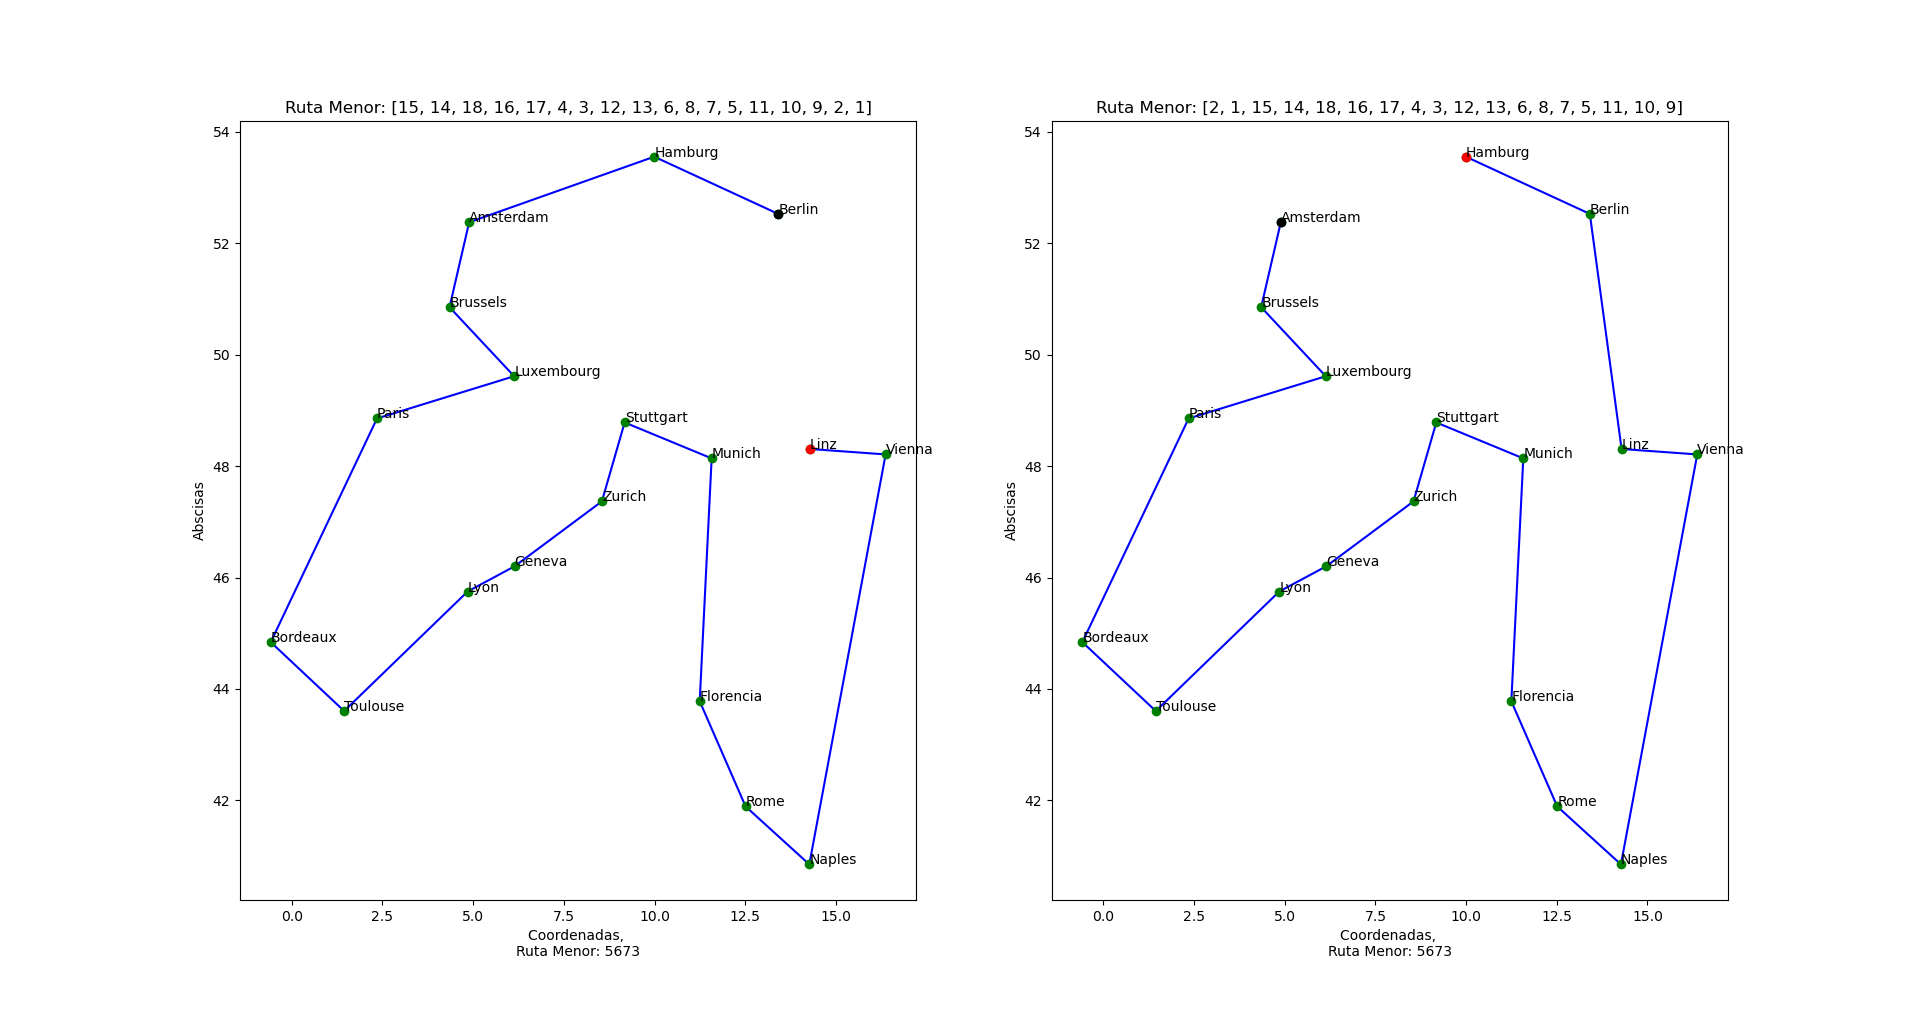
\includegraphics[width=1\textwidth]{C:/Users/anton/Documents/MCIA/UAQ _MCIA/Sem2_Computo_Evolutivo/Prac04TSPRestrictivo/pngs/finalPath1.png}
    \caption{Recorrido final: Selección Torneo.}
\end{figure}

\begin{figure}[H]
	\centering
    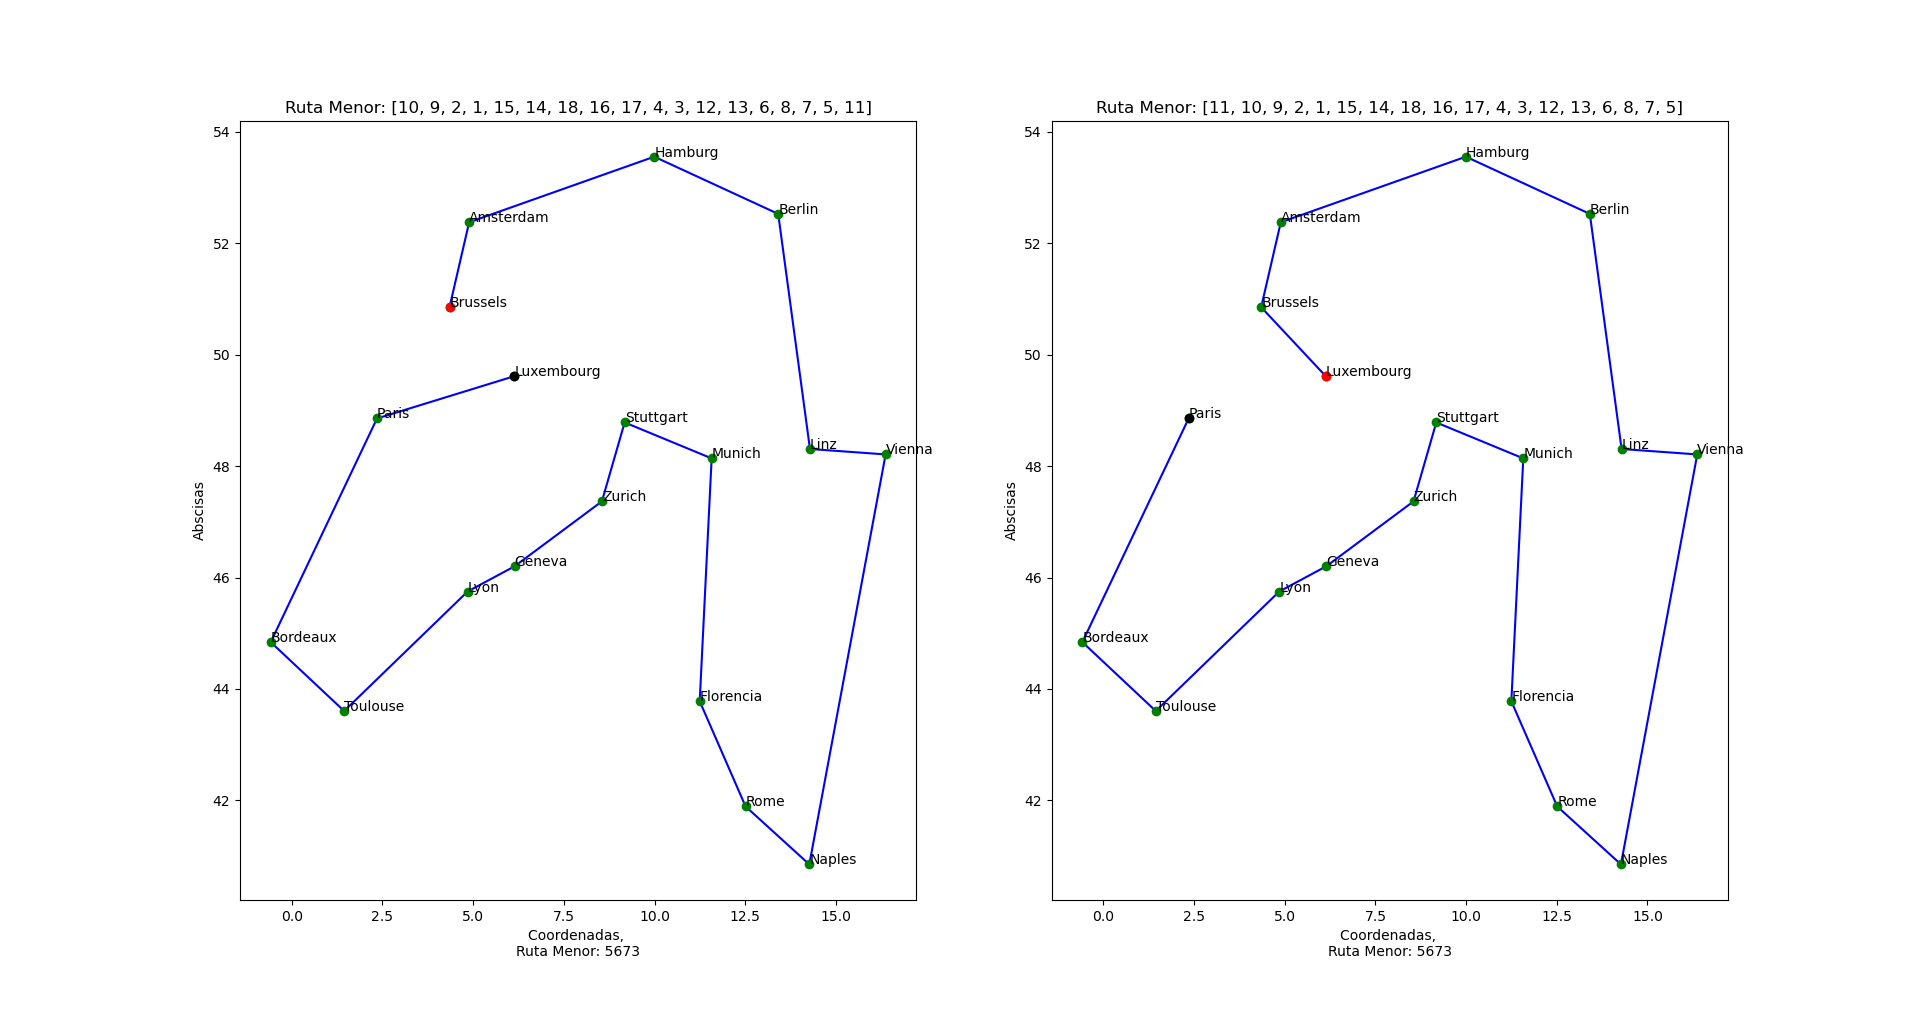
\includegraphics[width=1\textwidth]{C:/Users/anton/Documents/MCIA/UAQ _MCIA/Sem2_Computo_Evolutivo/Prac04TSPRestrictivo/pngs/finalPath.png}
    \caption{Recorrido final: Selección Rank.}
\end{figure}

Como se observa en las figuras es posible encontrar mas de una ruta corta si no se toma en cuenta el inicio de la ciudad. Ademas, como se ve en las figuras, las rutas son equivalentes si hacen el mismo recorrido pero iniciando en diferente ciudad.
\\\\
En la figura 7 se muestran cadenas con la misma distancia minima pero diferente orden, que muestran diferentes rutas minimas.

\begin{figure}[H]
	\centering
    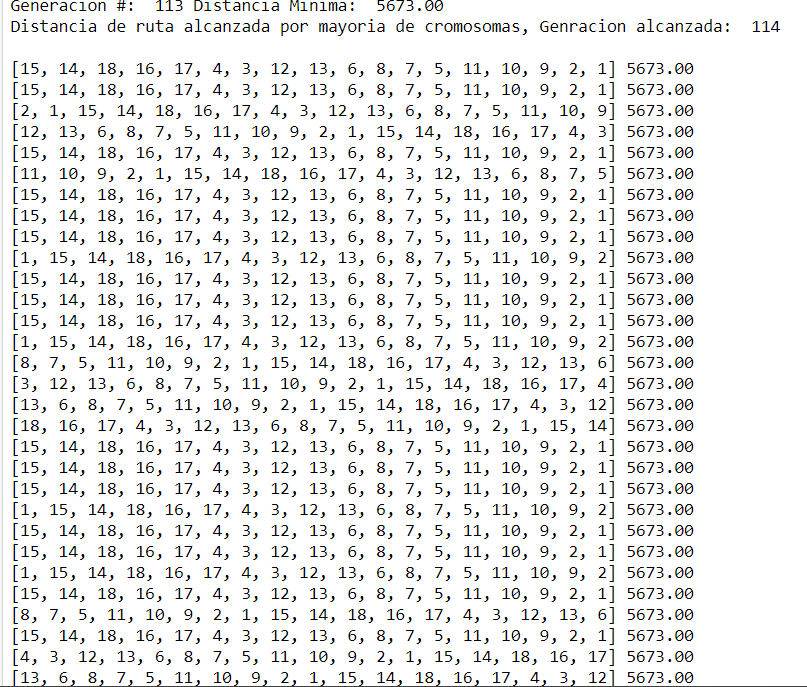
\includegraphics[width=1\textwidth]{C:/Users/anton/Documents/MCIA/UAQ _MCIA/Sem2_Computo_Evolutivo/Prac04TSPRestrictivo/pngs/conclusion02.png}
    \caption{Diferentes cadenas obtenidas con rutas minimas diferentes.}
\end{figure}


\begin{thebibliography}{0}
	\bibitem{nada1} http://reaxion.utleon.edu.mx/Reaxion\_a3\_numero\_2.pdf
	\bibitem{} https://es.wikipedia.org/wiki/Problema\_del\_viajante
	\bibitem{} http://www.cs.us.es/\~fsancho/?e=65
	\bibitem{} M. Yousaf., (2017), Genetic Algorithm for Traveling Salesman Problem with Modified Cycle Crossover Operator., Computational Intelligence and Neuroscience., Research Article., 7430125., 7 Pages.
\end  {thebibliography}

\section{Anexos}
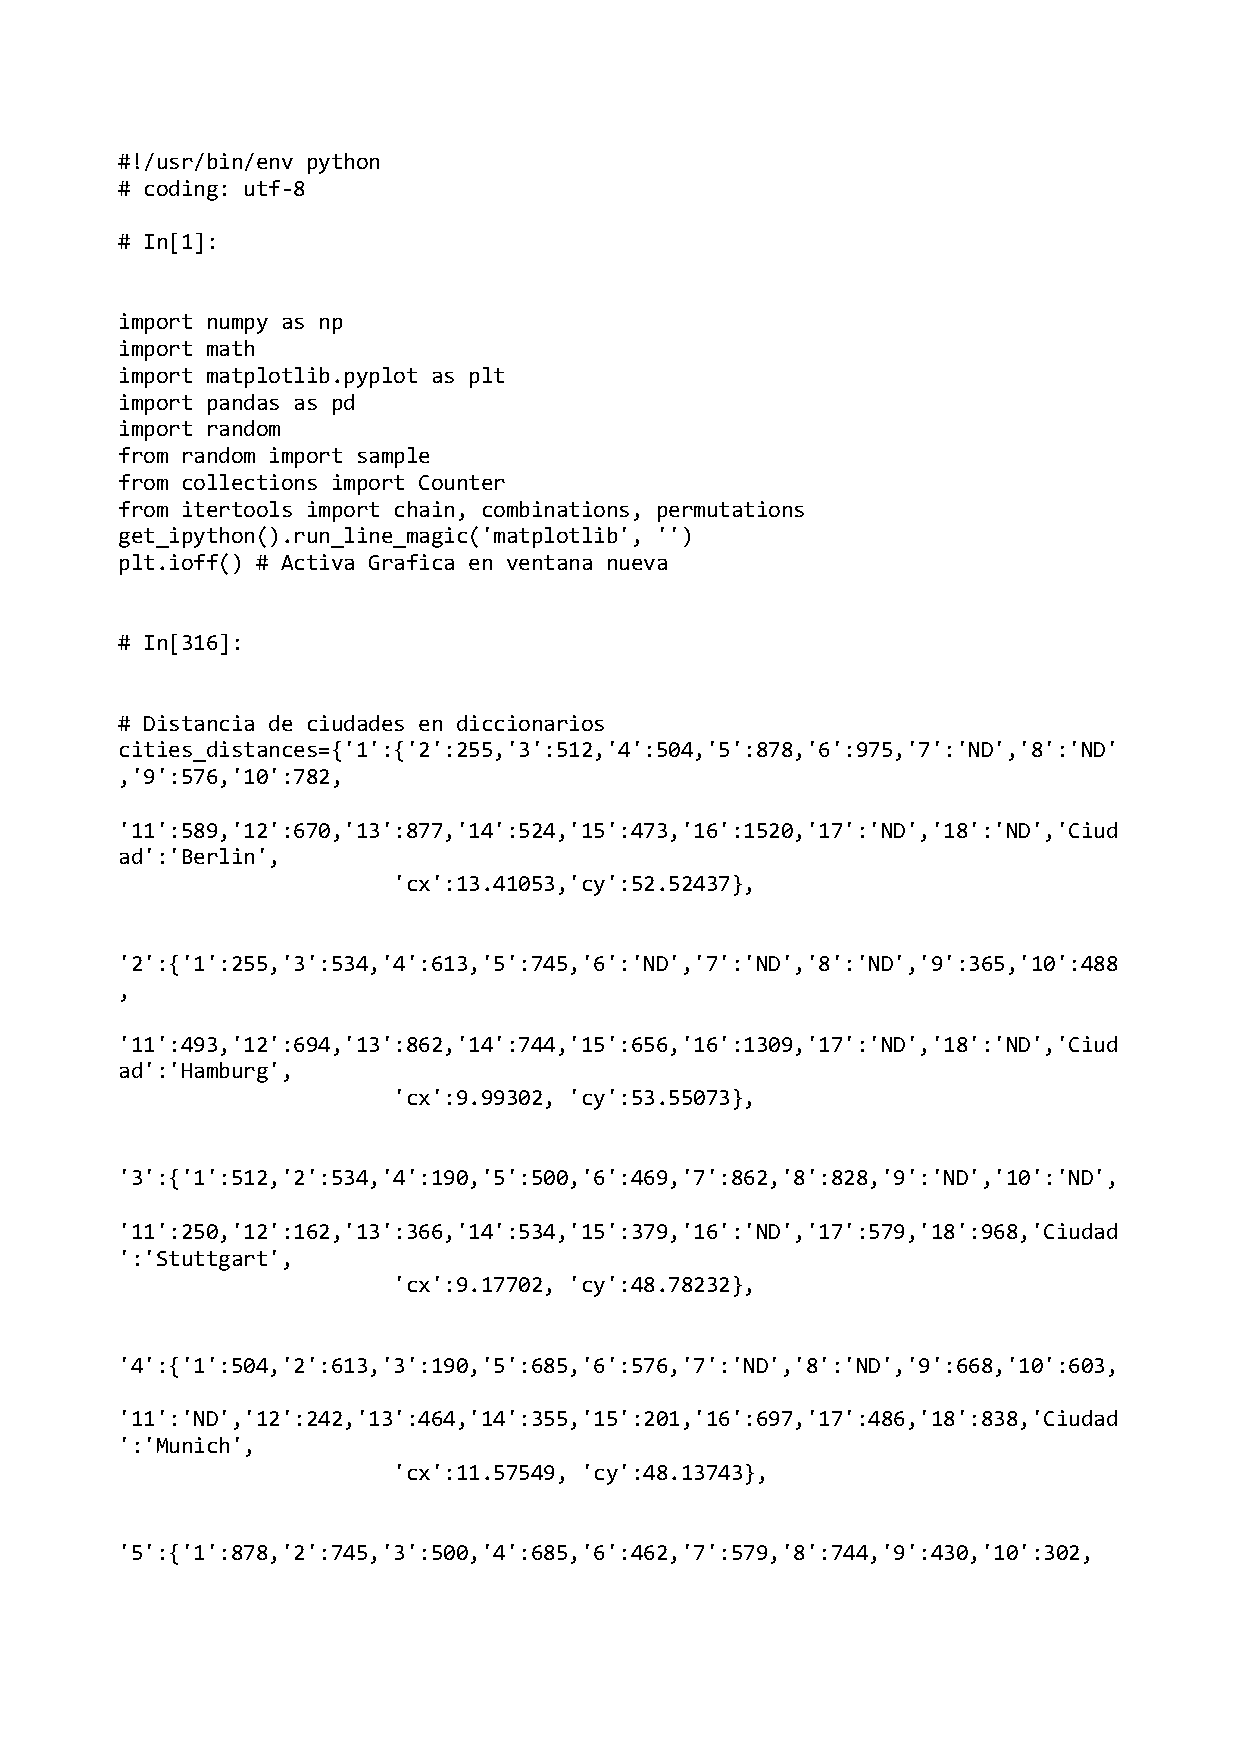
\includepdf[pages=-]{codTSPRestrictivo.pdf}

\end{document}